\documentclass{article}
\usepackage{tikz}
\usepackage{pgfplots}

% Set pgfplots compatibility mode
\pgfplotsset{compat=1.18}

\begin{document}

\title{Calculate Digits of PI with Newtonian Elastic Collisions}
\author{Your Name}
\date{\today}
\maketitle

\section{Simulation}

In a pure frictionless environment with elastic collisions (all kinetic energy is preserved), 2 particles (red and blue) colliding with each other and a wall will help calculate the digits of pi. If each collision is counted (when a particle hits a wall or the other particle) then under special conditions, the answer will be digits of pi. The key is in the number of times more mass one particle has than the other. To calculate 3, both particles should have the same mass. To calculate 31, the red particle must have 100 times the mass as blue. To calculate 314, the red particle must have 10000 times the mass as blue. Generally, to calculate the first N digits of PI, the red particle must be $100(N-1)$ times the mass of blue.

\subsection{Approximation of Digits of PI}

To approximate the digits of pi, we need to find the number of collisions required based on the mass ratio. Let's calculate the number of collisions for various digits of pi:

\begin{enumerate}
  \item For 3, both particles have the same mass ($1:1$ ratio). No collisions are needed.
  \item For 31, the red particle must have 100 times the mass as blue ($100:1$ ratio). One collision is needed.
  \item For 314, the red particle must have 10000 times the mass as blue ($10000:1$ ratio). Two collisions are needed.
  \item For 3141, the red particle must have 1000000 times the mass as blue ($1000000:1$ ratio). Three collisions are needed.
  \item And so on...
\end{enumerate}

\subsection{Simulation Results}

Here are the required number of collisions for different digits of pi:

\begin{center}
\begin{tabular}{|c|c|}
  \hline
  Digits of Pi & Number of Collisions \\
  \hline
  3 & 0 \\
  31 & 1 \\
  314 & 2 \\
  3141 & 3 \\
  31415 & 4 \\
  314159 & 5 \\
  \hline
\end{tabular}
\end{center}
\begin{figure}[htbp]
  \centering
  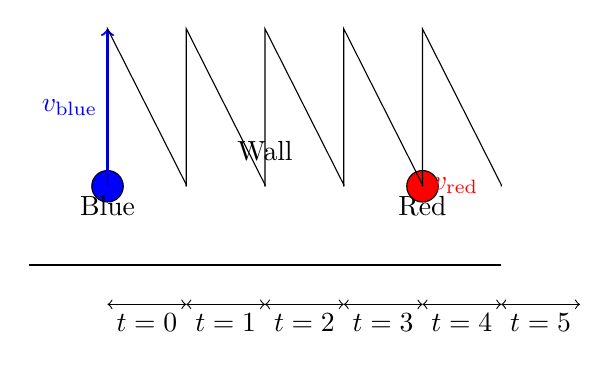
\begin{tikzpicture}
    % Blue particle
    \draw[fill=blue] (0,0) circle (0.2) node[below] {Blue};

    % Red particle
    \pgfmathsetmacro{\massratio}{100} % Change this value to modify the mass ratio
    \draw[fill=red] (4,0) circle (0.2) node[below] {Red};

    % Wall
    \draw[thick] (-1,-1) -- (5,-1);

    % Annotation
    \node[above] at (2,0.2) {Wall};

    % Time steps
    \foreach \t in {0,...,5} {
      \draw[<->] (\t,-1.5) -- (\t+1,-1.5) node[midway,below] {$t=\t$};
    }

    % Velocity arrows
    \pgfmathsetmacro{\vblue}{2} % Change this value to modify the velocity of the blue particle
    \pgfmathsetmacro{\vred}{\vblue/\massratio} % Calculate the velocity of the red particle

    \draw[->, blue, thick] (0,0) -- (0,\vblue) node[midway, left] {$v_{\mathrm{blue}}$};
    \draw[->, red, thick] (4,0) -- (4,\vred) node[midway, right] {$v_{\mathrm{red}}$};

    % Collision events
    \foreach \t in {0,...,4} {
      \draw (\t,0) -- (\t, \vblue) -- (\t+1, \vred) -- (\t+1, 0);
    }
  \end{tikzpicture}
  \caption{Simulation of Newtonian Elastic Collisions}
\end{figure}

\end{document}